\chapter{Quantum Optimal Control}\label{chap:3_Quantum_Optimal_control}

At time of writing, it is hard for me to imagine that there was a time when optimal control theory was not a widespread practice in the engineering of quantum technologies. 

\reminder{something something control objectives: state preparation, protection against decoherence, gate synthesis/optimisation, entanglement generation, enhanced measurements}

\reminder{what do you want to achieve $\rightarrow$ what is the quantitative formula for achieving this?}

Good citations to have in here: \cite{schirmer_complete_2001, koch_quantum_2022,glaser_training_2015}


\section{The structure of optimal control problems}\label{sec:3.1_structure_quantum_control}

The idea of an optimal control problem is simple: envision a target you want to achieve, cast it into some form of quantitative or abstract mathematical formula and then use said formula to derive the `best' path to get to said objective (`best' being ironically quite subjective in this case, as this can mean anything you'd like from `fastest' to `cheapest' to Backstreet Boys' iconic \emph{I want it that way}\cite{noauthor_backstreet_nodate}). However, as we are currently in the midst of a serious academic document, I will proceed by giving a slightly more precise and rigorous abstract definition for what optimal control really is.

In general, a control system in the context of optimal control theory is composed of a set of state functions $X: \R \rightarrow \R^n$, and a set of time-dependent control functions $U:\R \rightarrow \R^m$ and the optimal control problem consists of finding $x \in X$ and $u \in U$ that minimise some functional $C: X \cross U \rightarrow \R$ such that the constraint:
\begin{equation}\label{eq:control_ODE}
    \dot{x} = f(x, u),
\end{equation}
is satisfied almost everywhere. This is a very abstract description and just about any specific control problem can be expressed in terms of this formulation \cite{dalessandro_introduction_2021}. To gain more intuition, we can imagine a more concrete example where, \@~e.g. $U$ and $X$ are sets of continuous functions on the interval $[0, \tau]$ satisfying $x(0) = x_0$. In this scenario, $\tau$ could be a time interval during which we want to drive the system from an initial state $x_0$ to a final state $x_f$ using the control function $u(t)$. The choice of functional $C$ would have to capture the desired outcome of the protocol: that the state of the system after the driving $x(\tau)$ be equal to the target $x_f$. This can be done by choosing a distance metric that depends on only on the drive $u$ and is minimised when $x(\tau) = x_f$, \@~e.g.
\begin{equation}\label{eq:example_cost_func}
    C(u) = \norm{x(\tau)  - x_f}^2.
\end{equation}
The functional $C$ is often referred to in literature as the \emph{cost} or \emph{loss} function \cite{wald_statistical_1950} as it encodes the quality of the final protocol with respect to the desired outcome of the protocol. In that sense, we can imagine adding constraints to the problem that may increase the `cost' of the protocol output if they are not satisfied to some degree. For example, Eq.~\eqref{eq:example_cost_func} can be modified to include additional terms:
\begin{equation}\label{eq:example_cost_func2}
    C(u) = \gamma \norm{x(\tau)  - x_f}^2 + \int_0^{\tau} \norm{u(t)}^2 dt,
\end{equation}
where $\gamma$ is a penalty term on the final state that scales its importance relative to the additional second term, which is analogous to the cost in the energy required to achieve the final state. This updated cost function can be read as introducing a competition between the quality of the final state and the amount of energy expended to get it there, mediated by the value of $\gamma$. 

From the above, it is not hard to see that there is a lot of freedom in constructing a control problem given a target outcome and some constraints. To make things more concise, there are generally two fundamental questions that need to be addressed when designing control problems for a physical system\cite{glaser_training_2015}:
\begin{enumerate}
    \item What target states are accessible? (the question of reachability) 
    \item How can a target state be reached? (the question of control design)
\end{enumerate}

The first of these is concerned with the fundamental mathematical structure of control systems \cite{schirmer_complete_2001, dalessandro_introduction_2021, dirr_lie_2008} and binary answers to questions like whether or not a target state $x(\tau)$ be reached given some set of controls $U'$. The second is more often related to engineering challenges, preoccupied with the design of suitable control sequences in practice. While the focus of this thesis will be almost explicitly on answering (2) in the setting of quantum systems, the next section will include a brief overview of what it might take to answer (1) in order to give more context for how external controls might affect the structure of Hamiltonians.

\section{Quantum optimal control}\label{sec:3.2_Quantum_optimal_control}

\begin{figure}[t]
\centering
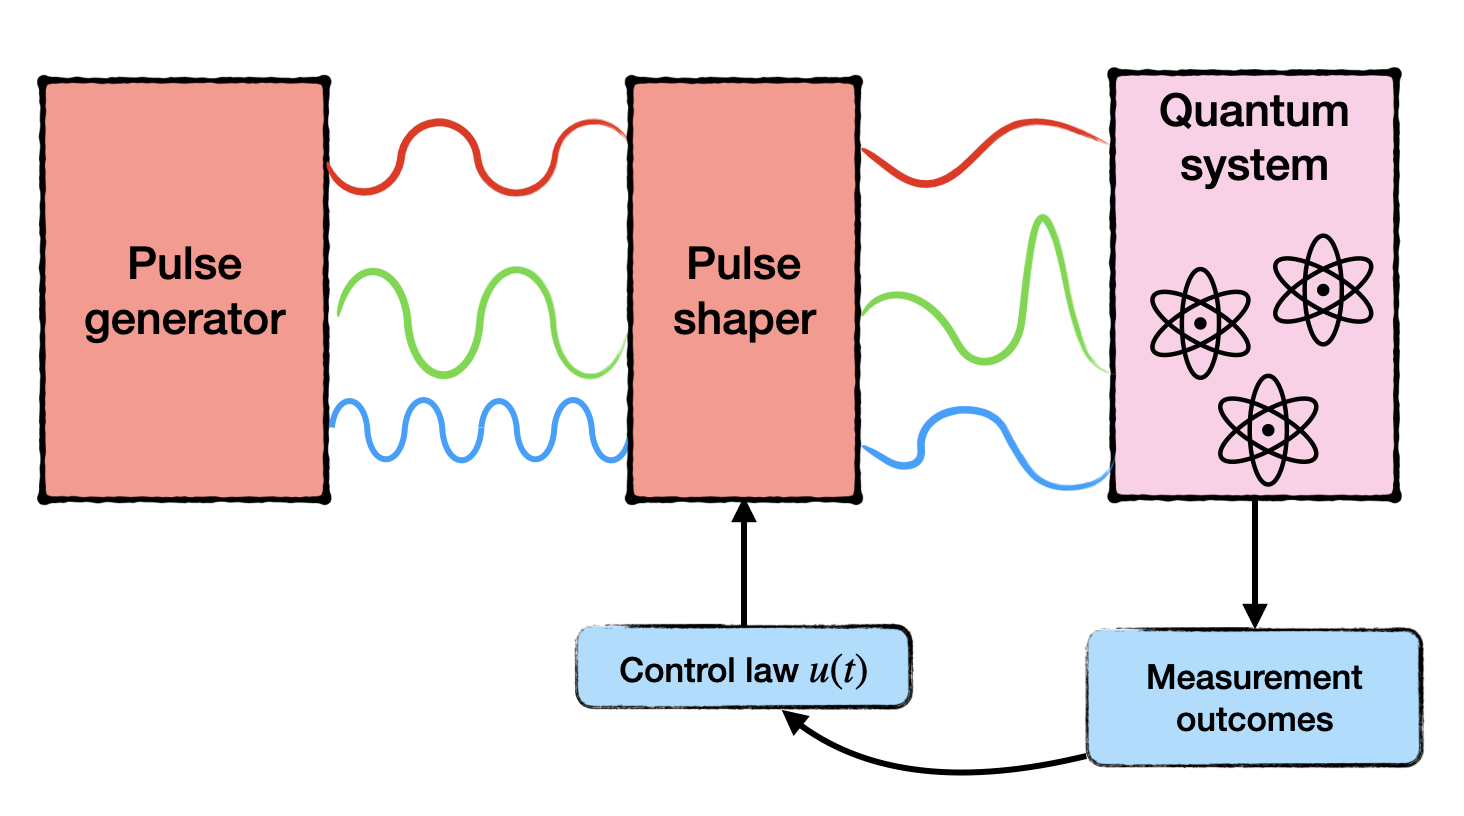
\includegraphics[width=0.9\linewidth]{images/optimal_control_placeholder.png} \caption{Placeholder}\label{fig:optimal_control}
\end{figure}

Having abstractly described what a control problem might look like, we can dive deeper into the more specific (and far more relevant to this thesis) field of \emph{quantum optimal control}. This is generally nothing more than the application of optimal control methods and ideas in the quantum setting, where the sets $X$ and $U$ are defined more concretely as quantum states and functions of parameterised Hamiltonians 

In the context we consider,  we employ quantum optimal control to optimise the function $f(\psi,\betabb)$ in the Schr\"odinger equation
\begin{equation}
\dot{\psi} = f(\psi,\betabb),
\label{eq:control_schroedinger}
\end{equation}

A commonly used cost function in state preparation is related  to the fidelity of the final, post-evolution state $\ket{\psi_f}$ with respect to the target state:
\begin{align} \label{eq:lossfunc}
    \mathcal{C}(\ket{\psi_f}) = 1 - \left|\braket{\psi_T}{\psi_f}\right|^2.
\end{align}

The full Hamiltonian of the control system is then:
\begin{align} \label{eq:h_optimal_control}
    H_{\beta}(t,\betabb)  = H_0(t) + \betabb(t)\mathcal{O}_{\rm opt}.
\end{align}

\subsection{Reachability}

\subsection{Design of controls}

\section{\acrref{CRAB}}

``Chopped random-basis quantum optimization" (CRAB) is a novel optimization method for quantum control problems. CRAB aims to optimize the control fields that drive the time evolution of quantum systems, particularly in problems where the control fields are piecewise constant. The method is based on the randomization of the control field basis and an efficient optimization algorithm.

The method in short:
\begin{enumerate}
    \item Initialization: Start by choosing an initial guess for the control fields, typically set to a constant value or initialized randomly.
    \item Random basis generation: Generate a random basis for each control field by selecting a set of random orthogonal vectors. The paper recommends using a Fourier basis and randomizing it through a linear transformation.
    \item Chopping: Divide the time interval of the control fields into several shorter subintervals (or chops). In each subinterval, the control fields are represented by a linear combination of the randomized basis functions.
    \item Optimization: Use a standard optimization algorithm to minimize the cost function. The cost function quantifies the deviation from the desired evolution of the quantum system. The optimization is performed with respect to the coefficients of the linear combinations, which represent the control fields in each subinterval.
    \item Iterative process: Iterate steps 2-4 until a satisfactory level of optimization is achieved.
\end{enumerate}

Advantages:

\begin{itemize}
    \item Enhanced exploration: The randomization of the control field basis allows for a more comprehensive exploration of the control landscape, which can lead to the discovery of better solutions.
    \item Improved convergence: The piecewise constant control fields enable the method to exploit local minima effectively, leading to faster convergence compared to other methods.
    \item Flexibility: The CRAB method can be applied to a wide range of quantum control problems, including those with constraints on the control fields or system parameters.
\end{itemize}

Disadvantages:

\begin{itemize}
    \item Additional complexity: The introduction of randomization and chopping adds complexity to the optimization process compared to traditional methods.
    \item Dependency on the optimizer: The efficiency and success of CRAB heavily depend on the choice of the optimization algorithm used in step 4.
    \item Convergence criteria: Determining an appropriate convergence criterion for terminating the iterative process can be challenging, as it may vary depending on the problem at hand.
\end{itemize}

Add in citations \cite{caneva_chopped_2011, muller_one_2022}

\section{\acrref{GRAPE}}

The ``Gradient Ascent Pulse Engineering" (GRAPE) algorithm is a widely used method for optimizing quantum control pulses in quantum computing and quantum information processing. The main goal of GRAPE is to determine control pulses that steer the quantum system from an initial state to a desired target state while minimizing a cost function. The algorithm iteratively refines the control pulses using gradient ascent optimization.

\reminder{can add some pseudocode across pages here}

\begin{algorithm}                     
\caption{GRAPE Algorithm}          
\label{findme}                          
\begin{algorithmic} [1]                   % enter the algorithmic environment
\REQUIRE    Here are a few variables \\
            variable 2 \\
            variable 3 
\ENSURE     this is the output \\
            output 2
\algstore{myalg}
\end{algorithmic}
\end{algorithm}

\begin{algorithm}                     
\begin{algorithmic} [1]                   % enter the algorithmic environment
\algrestore{myalg}
\STATE $some cool code here$
\STATE $some cool code here$
\STATE $some cool code here$
\STATE $some cool code here$
\end{algorithmic}
\end{algorithm}

\begin{enumerate}
    \item Initialization: Begin with an initial guess for the control pulses, which can be set to a constant value or initialized randomly.
    \item Propagation: Simulate the time evolution of the quantum system under the given control pulses to calculate the final state of the system.
    \item Cost function evaluation: Compute the cost function, which quantifies the deviation between the target state and the final state obtained in step 2. Common choices for the cost function are the fidelity or the infidelity between the two states.
    \item Gradient calculation: Compute the gradient of the cost function with respect to the control pulses. This is done by numerically evaluating the partial derivatives of the cost function with respect to each control pulse.
    \item Pulse update: Update the control pulses by following the gradient direction. This is typically done using a step size parameter that controls the magnitude of the pulse updates.
    \item Iterative process: Repeat steps 2-5 until the cost function reaches a satisfactory minimum value or a maximum number of iterations is reached.
\end{enumerate}

Advantages:

\begin{itemize}
    \item Robustness: GRAPE is known to be robust against local minima and typically converges to a global minimum for many quantum control problems.
    \item Efficiency: The algorithm is computationally efficient, as it only requires the calculation of the gradient of the cost function with respect to the control pulses.
    \item Wide applicability: GRAPE can be applied to a broad range of quantum control problems, including those involving constraints on the control pulses or system parameters.
\end{itemize}

Disadvantages:

\begin{itemize}
    \item Gradient calculation: The numerical calculation of the gradient can be challenging, particularly for systems with a large number of control pulses or complex dynamics.
    \item Convergence speed: The convergence rate of the GRAPE algorithm can be slow, especially if the initial guess for the control pulses is far from optimal.
    \item Dependency on the step size: The choice of the step size parameter can significantly affect the performance of the algorithm, with inadequate choices leading to slow convergence or oscillatory behavior.
\end{itemize}

Add in citations \cite{khaneja_optimal_2005}

\section{Optimisers}

\subsection{Powell optimisation}

\subsection{Dual-annealing}